% Chapter 21 -- Claim: Machine Learning Finds Hidden Alpha
% Requires: amsmath, amssymb, booktabs, array, tabularx, graphicx, tcolorbox (breakable, skins), hyperref or url.
% Defines the callout box only if the preamble has not.
\providecolor{fenavy}{HTML}{1B2A6B}
\providecolor{feshade}{HTML}{F3F5FA}
\makeatletter
\@ifundefined{callout}{%
  \newtcolorbox{callout}{breakable, enhanced,
    colback=white, colframe=gray!70, boxrule=0.5pt, arc=1mm,
    borderline west={2.5pt}{0pt}{gray!70},
    left=8pt, right=8pt, top=4pt, bottom=4pt}%
}{}
\makeatother

\chapter{Claim: Machine Learning Finds Hidden Alpha}
\label{ch:21}

Machine learning has transformed image recognition, translation and protein folding. The pitch to investors is that it can do the same for stock picking. Linear models, the argument runs, can only add up a handful of signals. Flexible models can find interactions and nonlinearities that humans never thought to look for, and with them, alpha that is hidden from everyone else.

The academic evidence gave the pitch real support. In 2020, Shihao Gu, Bryan Kelly and Dacheng Xiu reported that neural networks and regression trees roughly doubled the performance of leading regression-based strategies in predicting U.S. stock returns. Funds and ETFs branded with artificial intelligence followed.

Finance is a hard domain for machine learning. Signals are faint, data are short, and the patterns change as investors learn them. This chapter asks how much of the gain survives honest out-of-sample testing, realistic trading costs and the restriction to stocks that can actually be traded in size.

By the end of the chapter you will be able to:

\begin{itemize}
  \item state the return-prediction problem and describe the main model families: regularized regression, trees and ensembles, and neural networks;
  \item split data into training, validation and test samples in time order, and explain what each is for;
  \item measure success with the out-of-sample $R^2$, the Diebold--Mariano test and long--short portfolios, and explain why a tiny $R^2$ can be economically large;
  \item interpret a model with permutation importance, and explain the debate over the ``virtue of complexity'';
  \item state the three parts of the claim (statistical, hidden, economic) and summarize the evidence for each;
  \item judge a machine-learning strategy by its value-weighted, net-of-cost performance against a linear model on the same inputs.
\end{itemize}

\section{Foundations: supervised learning for return prediction}
\label{sec:21-foundations}

\textbf{The prediction problem.} For asset $i$ at the end of month $t$, a model maps a vector of characteristics $\mathbf{z}_{i,t}$, known at that time, to a forecast of next month's excess return:
\begin{equation}
  E_t[r_{i,t+1}] = g(\mathbf{z}_{i,t})
  \label{eq:21-g}
\end{equation}
Traditional models make $g$ linear, with a few characteristics chosen in advance. \textbf{Supervised machine learning} lets the data choose $g$ from a richer family and controls overfitting by holding back data to tune the model's complexity.

\textbf{The model families.}

\begin{itemize}
  \item \textbf{Ordinary least squares (OLS)} with many predictors fits noise. With $P$ predictors and $T$ observations, the in-sample fit improves mechanically with each added predictor.
  \item \textbf{Regularized regression} adds a penalty to the squared error. \textbf{Ridge} penalizes the sum of squared coefficients ($\lambda\sum_j\beta_j^2$), \textbf{lasso} the sum of their absolute values ($\lambda\sum_j|\beta_j|$), which sets some to zero, and the \textbf{elastic net} mixes the two.
  \item \textbf{Regression trees} split the data repeatedly on one characteristic at a time and predict the average return in each final group. A single tree overfits, so practitioners average many trees (\textbf{random forests}) or build them one after another, each correcting the last (\textbf{gradient boosting}). Tree depth controls how many characteristics can interact.
  \item \textbf{Neural networks} pass the inputs through layers of weighted sums and nonlinear functions. They can approximate almost any smooth function, but they have many parameters, depend on random initialization and need careful regularization: weight penalties, early stopping and averaging over several random \textbf{seeds}, the numbers that start the random initialization.
\end{itemize}

\textbf{Training, validation and testing.} The data are split in time (Figure~\ref{fig:21-split}). Models are fitted on a training sample, their tuning parameters (the penalty, the tree depth) are chosen on a later validation sample, and they are judged on a test sample that played no part in either step. Refitting as time passes keeps the split honest (Chapter 5).

\begin{figure}[htbp]
\centering
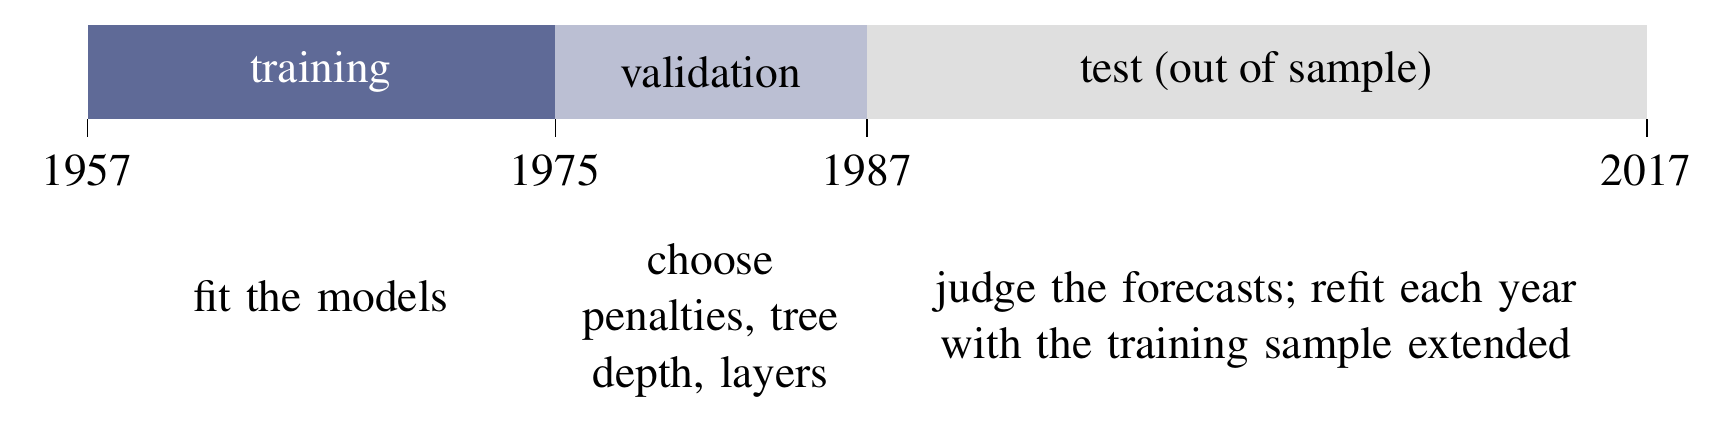
\includegraphics[width=0.9\linewidth]{images/fig21-1-split.png}
\caption{The time split in Gu, Kelly and Xiu (2020). Models are fitted on 1957--1974, their tuning parameters chosen on 1975--1986, and their forecasts judged on 1987--2016, a test period that played no part in fitting or tuning.}
\label{fig:21-split}
\end{figure}

\textbf{Measuring success.} Gu, Kelly and Xiu (2020) use an out-of-sample $R^2$ measured against a forecast of zero:
\begin{equation}
  R^2_{oos} = 1 - \frac{\sum (r_{i,t+1} - \hat{r}_{i,t+1})^2}{\sum r_{i,t+1}^2}
  \label{eq:21-r2}
\end{equation}
For individual stocks, a monthly $R^2$ of a few tenths of a percent is economically large (Figure~\ref{fig:21-gkx}). The \textbf{Diebold--Mariano test} checks whether one model's forecast errors are smaller than another's by more than chance. The economic test is a \textbf{long--short portfolio}: each month, buy the assets with the highest forecasts and sell those with the lowest.

\begin{figure}[htbp]
\centering
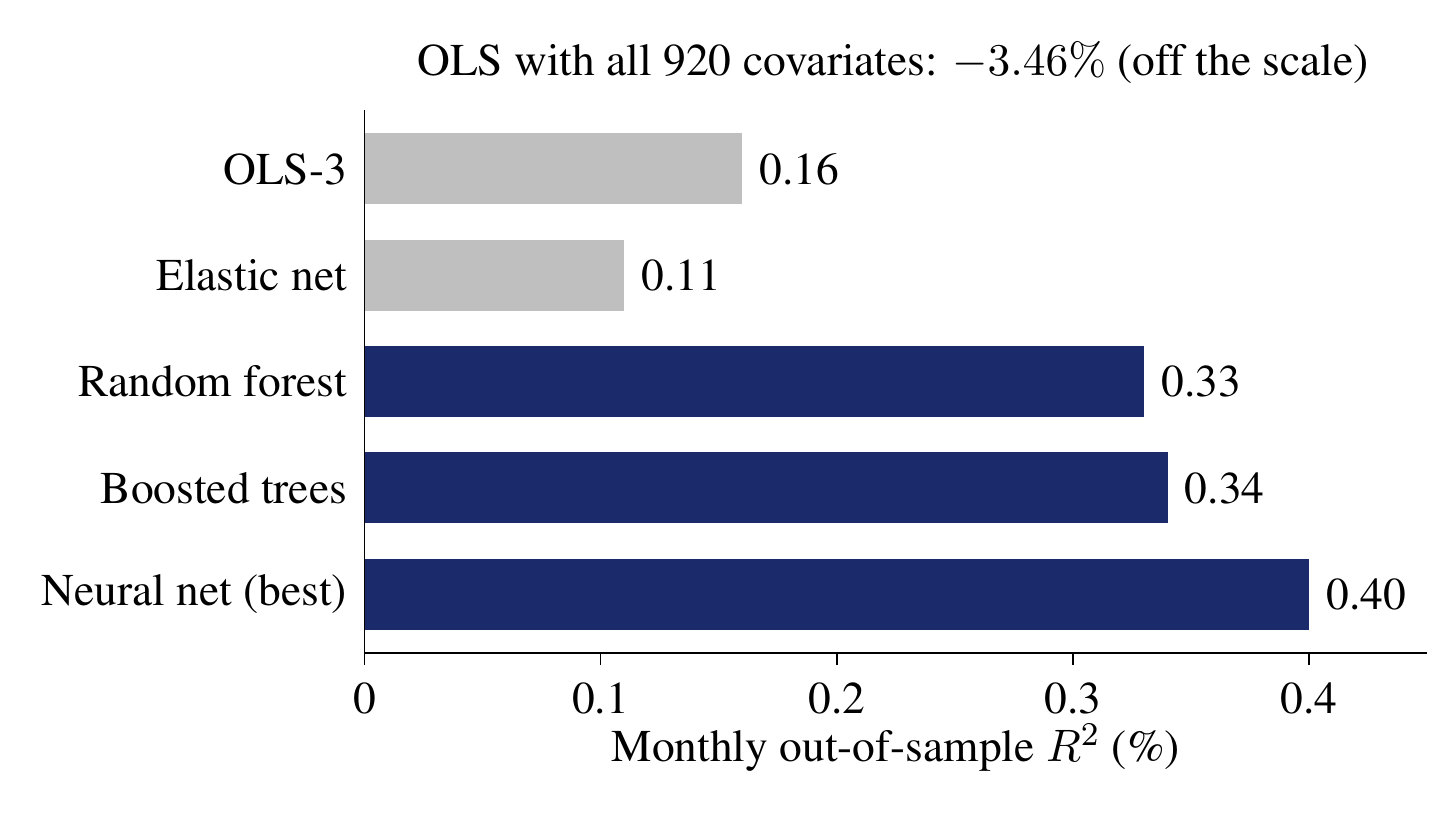
\includegraphics[width=0.85\linewidth]{images/fig21-2-gkx-r2.png}
\caption{Monthly out-of-sample $R^2$ for individual U.S. stocks, 1987--2016, from Gu, Kelly and Xiu (2020). Trees and neural networks roughly doubled the $R^2$ of a three-characteristic OLS model. OLS on all 920 covariates, at $-3.46\%$, was far worse than forecasting zero.}
\label{fig:21-gkx}
\end{figure}

\textbf{Worked example.} A stock's monthly return has a volatility of 10\%. A model that explains 0.4\% of its variance has forecasts with a volatility of $\sqrt{0.004} \times 10\% = 0.63\%$ a month.

\begin{itemize}
  \item If the forecasts are unbiased, the gap in expected return between a stock forecast one standard deviation above average and one forecast one standard deviation below is about 1.3\% a month, or more than 15\% a year.
  \item Applied across thousands of stocks, a tiny $R^2$ can support a profitable strategy.
  \item Most of that spread, however, may come from small, illiquid stocks that are costly to trade.
\end{itemize}

\textbf{Interpreting a model.} \textbf{Permutation importance} shuffles one input at a time, breaking its link to returns, and measures how much the forecast accuracy falls.

\textbf{Complexity.} Classical statistics warns against models with more parameters $P$ than observations $T$. Recent theory on ``benign overfitting'' shows that heavily over-parameterized models with a small ridge penalty can still forecast well out of sample. Kelly, Malamud and Zhou (2024) argued that this applies to return prediction.

\textbf{Further reading.} Hastie, Tibshirani and Friedman, \emph{The Elements of Statistical Learning}, and James, Witten, Hastie and Tibshirani, \emph{An Introduction to Statistical Learning} (regularization, trees, boosting, validation); Goodfellow, Bengio and Courville, \emph{Deep Learning}; Kelly and Xiu, ``Financial Machine Learning'' (\emph{Foundations and Trends in Finance}), and Nagel, \emph{Machine Learning in Asset Pricing}; L\'opez de Prado, \emph{Advances in Financial Machine Learning} (backtest overfitting in practice).

\section{How it works}
\label{sec:21-how}

A machine-learning return model has three ingredients: the inputs, the model and the discipline that keeps it honest.

\textbf{Inputs.} Academic studies use dozens to hundreds of stock characteristics: size, value, momentum, profitability, investment, volatility, liquidity and many accounting ratios. Most come from the anomaly literature of Chapters 8 to 12. Some studies add macroeconomic variables and let the model learn how the value of each characteristic changes with the economy.

\textbf{Model.} Where a linear model adds up characteristics with fixed weights, a tree or neural network can learn that momentum works differently in small and large stocks, or that high volatility hurts returns only beyond a threshold. These are the interactions and nonlinearities that the claim says are hidden.

\textbf{Discipline.} Flexibility is also the danger. A model with enough freedom will fit the noise in any training sample. The defences are:

\begin{itemize}
  \item a strict time split between training, validation and testing;
  \item penalties and early stopping, tuned on validation data only;
  \item averaging over random seeds and many models;
  \item a final test period long enough to separate skill from luck.
\end{itemize}

Three features of finance make the task harder than image recognition:

\begin{itemize}
  \item \textbf{The signal is weak.} Most of a stock's monthly return is unpredictable noise.
  \item \textbf{The data are few.} A century of monthly data is about 1,200 time periods.
  \item \textbf{The target moves.} Once investors learn a pattern, it tends to shrink (Chapter 10).
\end{itemize}

Finally, a forecast is only as valuable as the portfolio built from it. If the predictability lives in small, illiquid stocks, or requires trading half the portfolio each month, little of it reaches an investor.

\section{The claim}
\label{sec:21-claim}

\begin{callout}
\textbf{Claim.} Machine-learning models find return predictability that traditional linear models miss, and it can be turned into profitable portfolios.
\end{callout}

The claim has three parts, each of which can fail on its own:

\begin{itemize}
  \item \textbf{Statistical:} flexible models forecast returns out of sample better than linear models using the same inputs.
  \item \textbf{Hidden:} the gain comes from interactions or nonlinear effects, not from simply using more of the characteristics already known to predict returns.
  \item \textbf{Economic:} the gain survives trading costs and holds among stocks large enough to trade.
\end{itemize}

\section{The original evidence}
\label{sec:21-evidence}

\textbf{Gu, Kelly and Xiu (2020).} The landmark study used monthly CRSP returns for almost 30,000 U.S. stocks from March 1957 to December 2016, an average of more than 6,200 a month. Inputs were 94 stock characteristics, 8 macroeconomic predictors and 74 industry dummies, about 920 covariates once characteristics were interacted with macro variables. Models were trained on 1957--1974, validated on 1975--1986 and tested on 1987--2016.

\begin{center}
\small
\begin{tabularx}{0.9\linewidth}{@{}>{\raggedright\arraybackslash}X>{\raggedright\arraybackslash}p{0.35\linewidth}@{}}
\toprule
Model & Monthly out-of-sample $R^2$ (\%) \\
\midrule
OLS, all covariates & $-3.46$ \\
OLS-3 (size, book-to-market, momentum) & 0.16 \\
Elastic net & 0.11 \\
Random forest & 0.33 \\
Gradient-boosted trees & 0.34 \\
Neural networks (one to five layers) & 0.33 to 0.40 \\
\bottomrule
\end{tabularx}
\end{center}

A long--short decile portfolio sorted on neural-network forecasts earned an annualized Sharpe ratio of 1.35 value-weighted and 2.45 equal-weighted. The corresponding figures for the benchmark OLS model were 0.61 and 0.83. All methods agreed on the dominant signals: price trends (momentum, industry momentum, short-term reversal), liquidity (size, dollar volume, bid--ask spread) and volatility (total and idiosyncratic volatility, beta).

Two details matter for what follows. OLS with all covariates was a disaster, so regularization of some kind is essential. And the gap between equal-weighted and value-weighted results suggests that much of the profit comes from small stocks.

\textbf{Avramov, Cheng and Metzker (2023).} Avramov, Cheng and Metzker examined where machine-learning profits come from. Excluding microcaps, distressed stocks or periods of high market volatility considerably weakened profitability. Reasonable trading costs reduced it further, because the strategies had high turnover and took extreme positions.

\textbf{Kelly, Malamud and Zhou (2024).} Kelly, Malamud and Zhou proved that, in their framework, simple models with few parameters severely understate return predictability compared with complex models that have more parameters than observations. Empirically, they forecast the U.S. stock market with ridge regressions on thousands of random nonlinear transformations of standard market predictors, trained on as little as 12 months of data. They concluded that complexity is a virtue and that machine learning is justified for modelling expected returns.

\textbf{Nagel (2025).} Stefan Nagel showed that when the number of random features greatly exceeds a 12-month training window, the forecast becomes a weighted average of the training-window returns. The weights reflect how similar each past month's predictors are to today's, and in short windows that mostly means how recent the month is. The complex model therefore behaves like a volatility-timed momentum strategy. In artificial data with reversals instead of momentum, the same method still builds that strategy and does poorly. On this reading, the virtue of complexity is a strategy that happened to work, not new information extracted by the model.

The evidence supports the statistical part of the claim, at least for broad stock samples. It is weaker on the hidden part, because the models lean on well-known signals. It is weakest on the economic part.

\section{Replication lab: machine learning on a portfolio panel}
\label{sec:21-lab}

\begin{callout}
\textbf{Lab 21 at a glance.} \emph{Claim on trial:} machine learning finds return predictability that linear models miss, and it survives costs. \emph{Data:} a panel of 149 value-weighted portfolios from the Kenneth R. French Data Library (100 sorted on size and book-to-market, and 49 industries), with the Fama--French factors; the Goyal--Welch predictors for Part D. All are free. \emph{Code:} runs as a script (\texttt{python lab21.py}, or \texttt{python lab21.py -{}-fast}) or as a notebook (\texttt{lab21\_walkthrough.ipynb}) with a prediction prompt before each step.
\end{callout}

Lab 21 cannot use individual stocks, because CRSP is not free. Portfolios average away much of the noise in single stocks and leave out microcaps. The test is therefore closer to what a large investor can trade, but it is not the same test as Gu, Kelly and Xiu's.

Each month the lab computes ten characteristics for every portfolio, ranks them across portfolios and scales them to $[-1, 1]$:

\begin{itemize}
  \item average firm size, number of firms and book-to-market;
  \item last month's return, momentum and long-term reversal;
  \item volatility, beta, idiosyncratic volatility and the largest recent monthly return.
\end{itemize}

Two market variables, the market's past 12-month return and volatility, let the models change their view with conditions. The target is next month's return relative to the average portfolio that month, so the models compete on ranking, not on timing the market.

Five models compete:

\begin{itemize}
  \item OLS on size, value and momentum (OLS-3);
  \item OLS on all twelve inputs;
  \item elastic net;
  \item gradient-boosted trees;
  \item a three-layer neural network averaged over three random seeds.
\end{itemize}

Models are retrained every five years on all earlier data. Their tuning parameters are chosen on the preceding ten years, and the out-of-sample period starts in 1975.

The lab has four parts:

\begin{itemize}
  \item \textbf{Part A} compares out-of-sample $R^2$, Diebold--Mariano tests against OLS-3, and long--short portfolios that buy the top 10\% and sell the bottom 10\% of portfolios by forecast (Figures 21.3 and 21.4).
  \item \textbf{Part B} repeats the comparison for large portfolios only, for 1975--1999 and 2000 onward, and net of trading costs of 10, 25 and 50 basis points per unit of turnover (Figure 21.5).
  \item \textbf{Part C} reruns the network with one seed at a time and measures permutation importance on 2000 onward for models fitted before 2000 (Figure 21.6).
  \item \textbf{Part D} tests the virtue of complexity: ridge regressions on 2 to 1,200 random Fourier features of the Goyal--Welch predictors, with a 12-month rolling window, forecasting the market (Figure 21.7).
\end{itemize}

The command \texttt{python lab21.py -{}-source sim} tests the code on simulated data.

\textbf{What the simulated run shows.} The lab was run end to end only on simulated data. In the simulation, expected returns depend linearly on value and momentum, and nonlinearly on an interaction of size with momentum and on a volatility threshold. A flexible model should therefore win, and the results check that the code can detect a signal of that kind.

\begin{itemize}
  \item Out-of-sample $R^2$ was 0.14\% for OLS-3, 0.19\% for OLS on all inputs, 0.18\% for the elastic net, 0.21\% for gradient-boosted trees and 0.19\% for the network. Only the trees beat OLS-3 decisively (Diebold--Mariano $t = 3.6$). OLS on all inputs and the network managed $t = 2.0$.
  \item Before costs, long--short Sharpe ratios ranged from 1.12 (OLS-3) to 1.32 (trees). The trees also traded most.
  \item Among large portfolios, the trees kept a Sharpe ratio of 1.09 against 0.76 to 0.80 for the other models.
  \item At 25 bp per unit of turnover, OLS on all inputs had the highest Sharpe ratio (0.83), ahead of the trees (0.77). At 50 bp, the trees fell to 0.22 and OLS on all inputs held 0.43.
  \item With a single seed, the network's $R^2$ ranged from 0.16\% to 0.18\% and its Sharpe ratio from 1.17 to 1.32.
  \item All three models ranked momentum as the most important input; the trees also leaned on volatility, as the simulation intended.
  \item In Part D, where the simulated predictors carried almost no information, models with as many features as observations and a tiny ridge penalty produced an $R^2$ of about $-1{,}200\%$. With heavy shrinkage, $R^2$ stayed near zero at every level of complexity.
\end{itemize}

On real data the lab answers what the simulation cannot: whether real portfolios contain nonlinear structure that the flexible models find, and whether it survives costs.

\section{Stress tests}
\label{sec:21-stress}

\textbf{The universe.} The single biggest influence on machine-learning results is which assets are included. Gu, Kelly and Xiu's equal-weighted Sharpe ratio was almost twice the value-weighted one. Avramov, Cheng and Metzker found that removing microcaps and distressed firms considerably weakened profits. The lab's portfolio panel removes microcaps by construction and adds a large-portfolio subset.

\textbf{Trading costs.} Flexible models tend to trade more, because small changes in inputs can flip a forecast. In the simulated run, the model with the best gross Sharpe ratio fell behind a linear model at 25 bp per unit of turnover. Costs should be charged at the level the investor actually pays, and turnover reported alongside every Sharpe ratio (Chapter 6).

\textbf{Time.} Results from 1987--2016 include the years before many anomalies were published and arbitraged (Chapter 10). The lab splits the out-of-sample period at 2000.

\textbf{Tuning and seeds.} Neural networks depend on random initialization and on many choices: layers, penalties, learning rates and stopping rules. A result that holds for one seed or one configuration, but not for others, is closer to luck than to skill. Ensembling over seeds, as Gu, Kelly and Xiu did, helps, and the lab reports single-seed results to show the spread.

\textbf{Researcher degrees of freedom.} Every published model is the survivor of many tried. The tuning sample controls overfitting within one design, but not the choice among designs (Chapter 4).

\textbf{Complexity in timing.} Kelly, Malamud and Zhou's result depends on the window, the penalty and the predictors. Nagel's reinterpretation implies a sharp test: if the complex model's timing signal is close to a simple volatility-scaled momentum rule, the complexity adds little. Exercise 8 runs that comparison.

\section{Verdict}
\label{sec:21-verdict}

\begin{callout}
\textbf{Verdict: weakens} (as of October 2026). The statistical part of the claim holds. In broad samples of U.S. stocks, regularized nonlinear models forecast returns out of sample better than linear models with a few characteristics, and the improvement is too large and consistent to be luck (Gu, Kelly and Xiu 2020). The other two parts are much weaker.
\end{callout}

\begin{itemize}
  \item \textbf{Not very hidden.} The models rely mostly on signals already known (momentum, short-term reversal, size, liquidity and volatility). Much of the gain comes from combining many such signals with appropriate shrinkage, which a well-regularized linear model also captures in part.
  \item \textbf{Not easily captured.} The economic gains are concentrated in small and distressed stocks and in volatile periods, and they shrink after realistic trading costs (Avramov, Cheng and Metzker 2023). The gap between equal-weighted and value-weighted results points the same way.
  \item \textbf{Complexity disputed.} The virtue of complexity in market timing may be a volatility-timed momentum strategy in disguise (Nagel 2025).
\end{itemize}

Machine learning is a better tool for an old job, not a source of hidden alpha. The verdict would move to \emph{survives} if value-weighted, net-of-cost machine-learning portfolios beat regularized linear ones among large stocks, out of sample after 2016, by a significant margin.

\section{What investors can use}
\label{sec:21-investors}

\begin{itemize}
  \item \textbf{Machine learning is a better blender, not a crystal ball.} Its proven value is in combining many known signals with care about overfitting. Expect modest improvements over a well-built linear multi-factor model, not a new source of returns.
  \item \textbf{Ask where the returns come from.} A strategy whose edge sits in microcaps, in the short side or in months of market stress may not be available at scale or after costs.
  \item \textbf{Insist on the net, value-weighted number.} Equal-weighted, gross-of-cost backtests flatter flexible models most.
  \item \textbf{Treat interpretability as a risk control.} If a manager cannot say which signals drive the forecasts, it is impossible to judge whether they will persist.
  \item \textbf{Expect decay.} Signals published in the academic literature lose part of their power after publication (Chapter 10). A model trained on them inherits the decay.
\end{itemize}

\textbf{Questions to ask a manager who sells machine-learning strategies:}

\begin{itemize}
  \item What is the out-of-sample period, and how often were the model and its tuning changed during it?
  \item How do results compare with a linear model on the same inputs, net of costs and value-weighted?
  \item How much of the return comes from the 20\% smallest stocks, and from the short side?
  \item What is the monthly turnover, and what trading costs are assumed?
  \item How much do results change with the random seed or with small changes to the training window?
\end{itemize}

\begin{callout}
\textbf{What Failed: the AI fund that trailed the index.} In 2017 the AI Powered Equity ETF (ticker AIEQ) launched as the first exchange-traded fund run by artificial intelligence. Its manager, EquBot, used IBM Watson to process news, filings and market data and to monitor tens of thousands of models. By January 2022 the fund was up 57\% since inception, while the S\&P 500 total return index was up 84\% over the same period (Tech Brew 2022). Assets were about \$150 million. The models were sophisticated; the difficulty was the task. Stock returns carry little signal, the competition for it is intense, and a model that learns from the past is always learning about a market that has already moved on.
\end{callout}

\section{Open questions}
\label{sec:21-open}

\begin{itemize}
  \item \textbf{Does the edge survive among large stocks?} The strongest machine-learning results come from broad samples dominated by small stocks. How much remains in the largest 500 or 1,000?
  \item \textbf{Hidden or known?} Do flexible models find genuinely new interactions, or mostly better ways to combine momentum, volatility and liquidity?
  \item \textbf{Complexity or momentum?} Is the virtue of complexity in market timing a general result or, as Nagel argues, a disguised volatility-timed momentum strategy?
  \item \textbf{New models and new data.} Chapter 22 asks the parallel question for time-series foundation models, and Chapter 23 for language models applied to news.
\end{itemize}

\section*{Exercises}
\addcontentsline{toc}{section}{Exercises}

\subsection*{Conceptual (all readers)}

\begin{enumerate}
  \item A model has a monthly out-of-sample $R^2$ of 0.3\% on stocks with 12\% monthly volatility. What is the standard deviation of its forecasts? What expected return gap separates stocks forecast one standard deviation above and below average?
  \item Explain why OLS with 920 covariates had an out-of-sample $R^2$ of $-3.46\%$ in Gu, Kelly and Xiu (2020), while OLS with three characteristics had $+0.16\%$.
  \item A gradient-boosted model uses trees of depth 1. Can it capture an interaction between size and momentum? What about depth 2?
\end{enumerate}

\subsection*{Lab extensions (technical readers)}

\begin{enumerate}
  \setcounter{enumi}{3}
  \item Part A: run on real data. Is the Diebold--Mariano statistic of the best nonlinear model against OLS-3 above 2?
  \item Compare the long--short Sharpe ratio of each model on all portfolios and on large portfolios only. Which model loses most?
  \item At what cost per unit of turnover does the best model's long--short Sharpe ratio fall below that of OLS-3?
  \item Part C: rank the characteristics by importance for the trees and for OLS. Do the flexible models rely on anything the linear model ignores?
  \item Part D: compute a volatility-scaled momentum rule for the market (last 12 months' return divided by trailing volatility) and correlate its timing signal with the complex model's forecasts. How much of the complex model's performance does the simple rule reproduce?
  \item Gu, Kelly and Xiu report much higher Sharpe ratios for equal-weighted than for value-weighted portfolios. What does that suggest about where the predictability lives, and about whether investors can capture it?
  \item A start-up claims its deep-learning model earned a Sharpe ratio of 3 in a backtest over 2010--2024. List the questions you would ask before investing.
\end{enumerate}

\section*{References}
\addcontentsline{toc}{section}{References}

\begin{itemize}
  \item Avramov, D., Cheng, S. and Metzker, L. (2023). Machine Learning vs.\ Economic Restrictions: Evidence from Stock Return Predictability. \emph{Management Science} 69(5): 2587--2619.
  \item Gu, S., Kelly, B. and Xiu, D. (2020). Empirical Asset Pricing via Machine Learning. \emph{Review of Financial Studies} 33(5): 2223--2273.
  \item Kelly, B., Malamud, S. and Zhou, K. (2024). The Virtue of Complexity in Return Prediction. \emph{Journal of Finance} 79(1): 459--503.
  \item Nagel, S. (2025). Seemingly Virtuous Complexity in Return Prediction. NBER Working Paper 34104.
  \item Tech Brew (2022). How the World's First AI-Managed ETF Stacks Up Almost Five Years Later. January 26.
\end{itemize}

\textbf{Data:} Kenneth R. French Data Library: 100 Portfolios Formed on Size and Book-to-Market (10 $\times$ 10); 49 Industry Portfolios; Fama/French 3 Factors. Goyal--Welch predictor data (Amit Goyal's website), for Part D.
